% Chapter 3

\chapter{Propuesta de aplicación} % Main chapter title
% \chapter{Propuesta de aplicación de modelos \glsentrytext{nlp} para el desarrollo de labores de inteligencia en escenarios de ciberterrorismo} % Main chapter title

\label{chap:proposal} % For referencing the chapter elsewhere, use \ref{Chapter1} 

%----------------------------------------------------------------------------------------

\newcommand{\nmodels}{$n$ \todo{?`cuantos modelos?}}

La propuesta consta de a aplicación de modelos de \glsentrytext{nlp} para el desarrollo de labores de inteligencia en escenarios de ciberterrorismo por medio de \nmodels modelos, pensados para el análisis de texto en redes sociales como Twitter en aras de realizar un perfilado de ciber-criminales potenciales, esto por medio de \gls{nlp}, de donde se parte varias metodologías que hacen uso de tecnologías \mbox{Estado-del-Arte}.

\section{Entendimiento del negocio (Business understanding)}
\todo{Pendiente}

\section{Adquisición de datos (Data acquisition)}
\todo[inline]{Incluir proceso de recolección por el API de Twitter o usando los datasets que estan en Archive}

\section{Modelamiento (Modelling)}
Como parte de la propuesta se proponen \nmodels modelos para tratar diferentes aspectos en perfilado de donde se representan los diferentes modelos en la \figureref{fig:proposal-arch}.

\begin{figure}[H]
  \centering
  % \missingfigure{Hacer la arquitectura en yEd}
  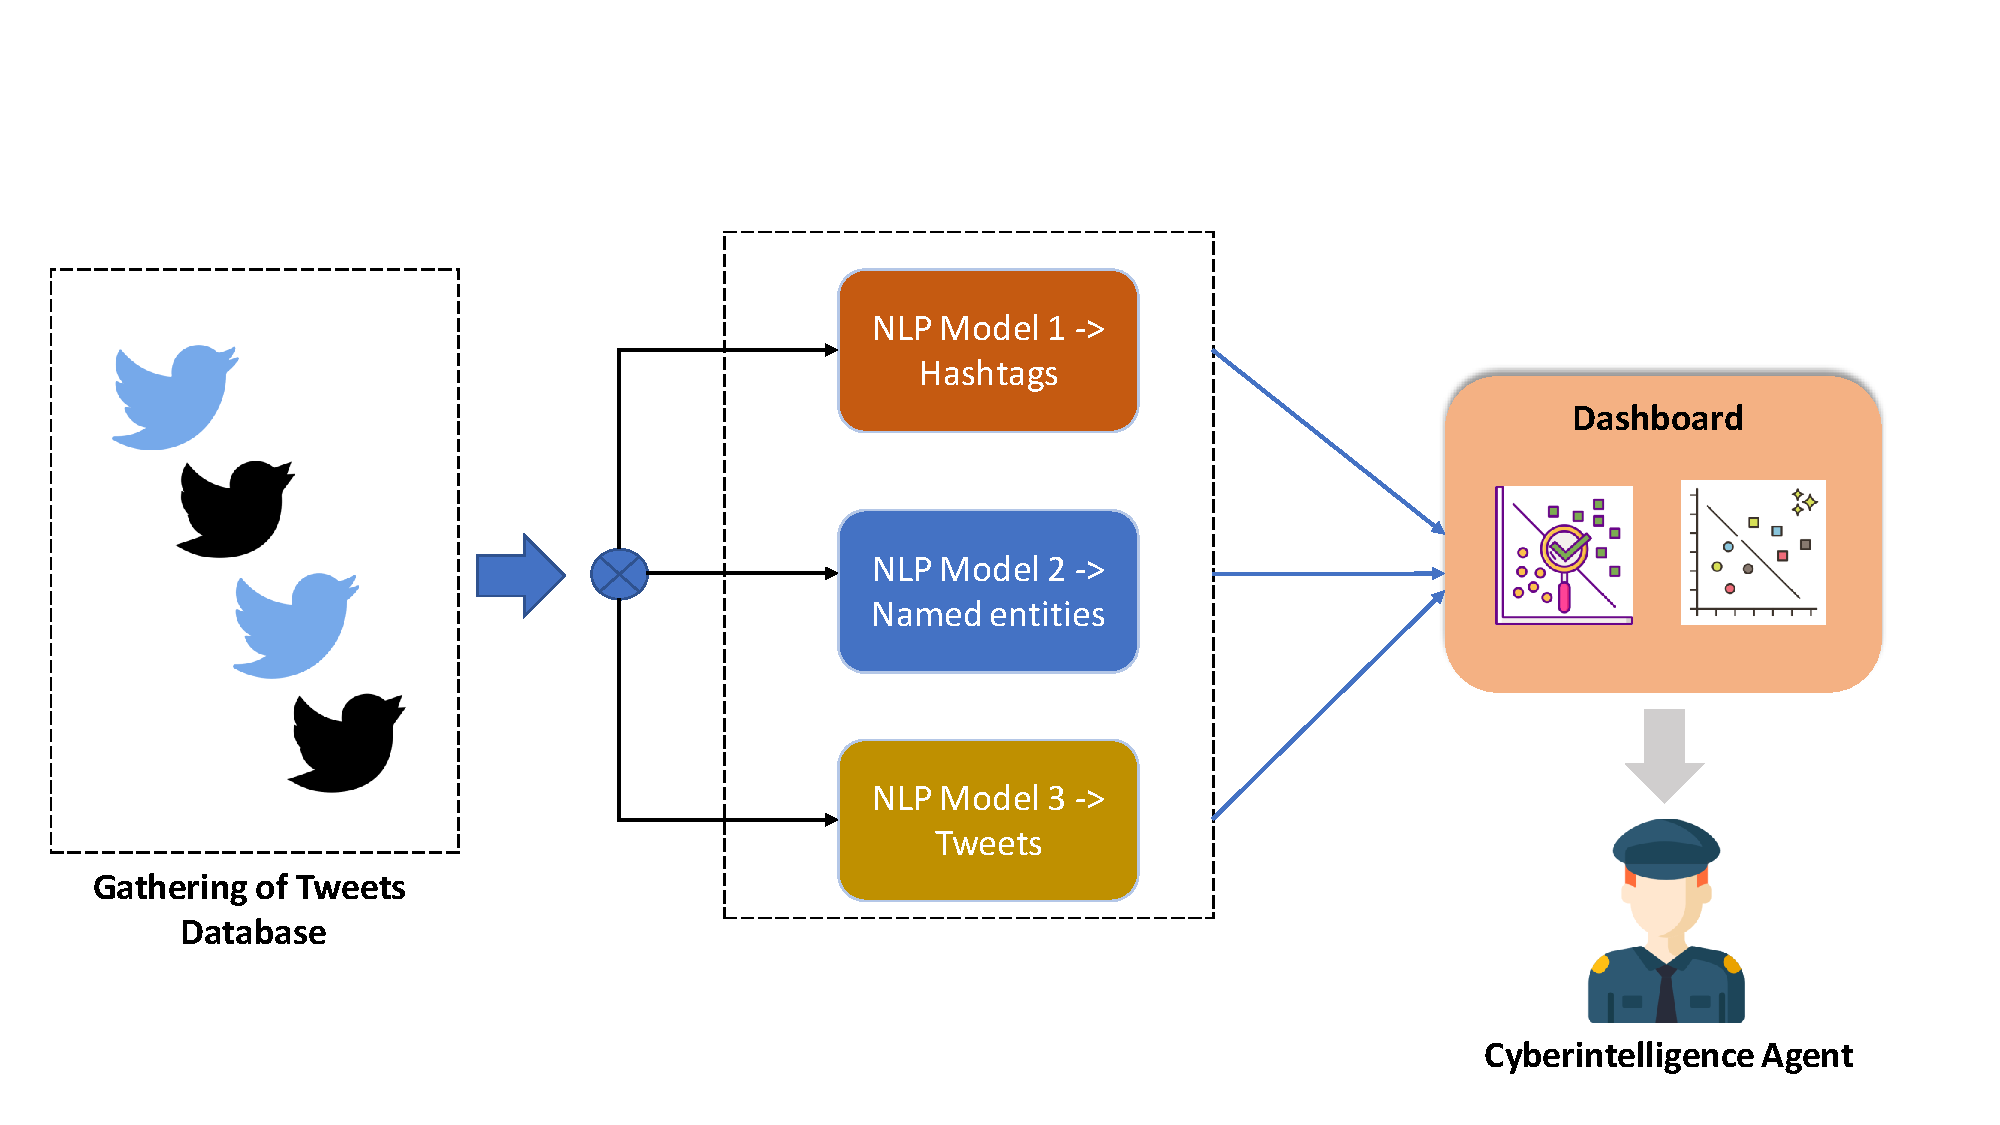
\includegraphics[width=\textwidth]{Figures/general-architecture.pdf}
\decoRule
\caption[Arquitectura de propuesta]{Arquitectura de propuesta.}
\label{fig:proposal-arch}
\end{figure}

\subsection{Modelo 1: Predicción de etiquetas de Twitter con modelos lineales} \label{sec:twitter-prediction}
En Twitter, las publicaciones que se realizan tienen la posibilidad de incluir menciones de temas de tendencia por el conocido \emph{hashtag}, escrito como \texttt{\#Tema}, y tiene la gran utilidad de realizar una mención explicita del tema que se quiere tratar y donde además la tarea de encontrar textos directamente relacionados con un tema son fácilmente localizables.

Así mismo, en la literatura de \gls{nlp} es muy común el uso de diferentes representaciones de palabras o conjuntos de palabras. Una representación de palabras típicas es por medio de los \gls{bow}, donde se establece un diccionario de palabras de tamaño $N$, y donde cada palabra tiene un vector que lo representa. A cada palabra se le asigna un identificador único en ese diccionario, por lo que existiría una traducción de palabra a identificador y una secuencia de palabras para poder ser recuperado por medio del índice, como se muestra en la \equationref{eq:bow-repr1} y la \equationref{eq:bow-repr2}.
\begin{equation} \label{eq:bow-repr1}
  \text{word2idx} = \Big\{(\text{word}_i, i) : \forall i \in \{1, \ldots, N\} \Big\}
\end{equation}

\begin{equation} \label{eq:bow-repr2}
  \text{idx2word} = \Big[\text{word}_i\Big], \forall i \in \{1, \ldots, N\}
\end{equation}

Otra representación común en \gls{nlp} es la de \gls{tfidf}, que se divide en dos partes, expresadas en las \equationref{eq:tf-repr}, la \equationref{eq:idf-repr} y la composición de ambas en la \equationref{eq:tfidf-repr}, $D$ es el corpus de palabras. Este consiste en penalizar palabras que ocurren mucho en un documento pero no mucho en el corpus o bien de penalizar la palabras que se repiten poco en un documento pero se repiten mucho en el corpus, por lo que un punto medio entre ambos es recompensado.

\begin{equation} \label{eq:tf-repr}
  \text{tf}(t,d) = \text{Frecuencia del termino (o n--grama) } t \text{ en el documento } d
\end{equation}

Existen diferentes variaciones para realizar representar el conteo de términos \textbf{tf} de forma normalizada, como se representa en el \tableref{table:tf}.

\begin{table}[h!]
\centering
\begin{tabular}{|l|l|} \hline
  \textbf{Esquema}          & \textbf{Peso de tf} \\ \hline
  Binario                   & $0, 1$ \\ \hline
  Conteo directo            & $f_{t, d}$ \\ \hline
  Frecuencia de términos    & $f_{t, d} / \sum_{t' \in d}f_{t', d}$ \\ \hline
  Normalización logarítmica & $1 + \text{log}(f_{f, d})$ \\ \hline
\end{tabular}
\caption{Variaciones de \textbf{tf}}
\label{table:tf}
\end{table}

\begin{equation} \label{eq:idf-repr}
  \text{idf}(t, D) = \text{log}\Bigg( \frac{N}{|\{d \in D : t \in d\}|} \Bigg) ; N = |D|
\end{equation}

\begin{equation} \label{eq:tfidf-repr}
  \text{tf-idf}(t, d, D) = \text{tf}(t, d) \cdot \text{idf}(t, D)
\end{equation}

\subsubsection{Creación del Corpus de palabras}
Debido a que los textos que se encuentran en Twitter no tienen forma estructurada es necesario realizar un preprocesamiento de cada post recolectado para luego contar la frecuencia de cada palabra dentro del corpus y así establecer las primeras $N$ palabras mas usadas que van a componer el corpus de palabras.

Para realizar el preprocesamiento de cada texto se hacen los siguientes pasos:
\begin{enumerate}
\item Convertir todas las palabras a minúscula (e.g. \mbox{``LaTeX'' $\rightarrow$ ``latex''})
\item Reemplazar todos los caracteres especiales de texto a espacios en blanco (e.g. \mbox{``\texttt{@;,:\textbackslash n\textbackslash t\textbackslash r}'' $\rightarrow$ ``\textvisiblespace \textvisiblespace \textvisiblespace \textvisiblespace \textvisiblespace \textvisiblespace \textvisiblespace''})
\item Remover todos los símbolos extraños, es decir todo lo que no sean numeros, ni letras ni los simbolos que se encuentran normalmente en tweets (e.g. \mbox{``\texttt{\%()\*\&\$!\^}'' $\rightarrow$ ``''})
\item Remover todas las \emph{stopwords}, que son palabras que no añaden ningún valor semántico al texto \\ (e.g. \mbox{``las palabras son una forma de expresarnos'' $\rightarrow$ ``palabras forma expresarnos''})
\end{enumerate}

Luego se realiza un conteo de todas la palabras presentes dentro del corpus de donde se sacan las $N$ primeras palabras para incluirlas en el \gls{bow}.

Luego de esto se generan las etiquetas (o \emph{tags} en ingles) que se toman directamente de los textos de entrenamiento, de estos también se les realiza un conteo, que servirán para la predicción de las etiquetas según el contenido del texto.

\subsubsection{Conversión de textos a vectores}
Para realizar la conversión de textos a vectores y así poder representar un texto como un vector se procede a primera realizar una generación de identificadores para cada palabra de manera como se describió en el inicio de la \sectionref{sec:twitter-prediction}.

La manera en que se representa un texto en forma de vector $\vs$ es por medio de la sumatoria de los vectores que representan cada palabra como se representa en la \equationref{eq:bow-word-vector-sum}, recuérdese que $\ve^{(i)}$ es un vector con un $1$ en la posición $i$ y ceros en el resto del vector.

\begin{equation} \label{eq:bow-word-vector-sum}
  \vs = \mathlarger{\mathlarger{\sum}}_{(\text{word}, i) \in \text{word2idx}} \ve^{(i)}, \text{word} \in d
\end{equation}

\subsubsection{Generación del conjunto de entrenamiento, validación y pruebas}
Para la generación de los conjuntos se toman las sumatorias generadas de cada tweet en su forma de vector y se coloca en una matriz de $\mT^{m \times N}$, donde $m$ son el numero de muestras de Twitter y $N$ el tamaño del Corpus.

\subsubsection{Clasificador de regresión logística}
La regresion logistica hace parte de uno de los algoritmos mas importantes en \gls{ai}, esta consiste en procesar la entrada de un modelo, que para el caso actual es lineal, que se procesa con una serie de hiper-parámetros que se denominara $\vtheta$ y la entrada del modelo como $\vx$. Se tiene que al realizar una regresión con este modelo se calcula $\vtheta^{\top} \vx$, que da como resultado un valor en $\R$ con rango indefinido. La regresión logística simbolizada como $\sigma(x)$, conocida como la función \emph{sigmoide} que es una función que para una entrada $x$ de dominio $(-\infty, \infty)$ se tenga un rango de $(0, 1)$, la \equationref{eq:logits-formula} define la función.

\begin{equation} \label{eq:logits-formula}
  \sigma(x) = \frac{1} {1 + \exp(-x)}
\end{equation}

Equivalentemente, la regresión logística con modelos lineales se calculan como $\sigma(\vtheta^{\top} \vx)$ y permite realizar un suavizado de la regresión de forma mitiga parte de los problemas de \gls{overfitting} y \gls{bias}, como se muestra en la \figureref{fig:logits-example}.

\begin{figure}[H]
  \centering
  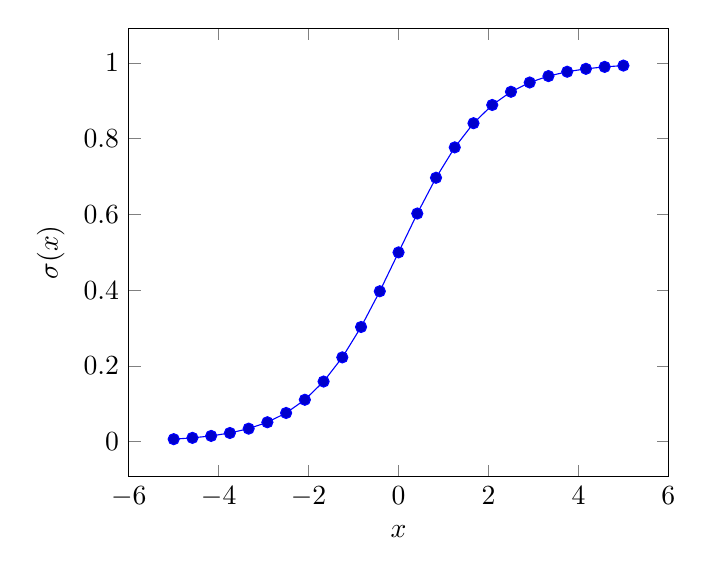
\begin{tikzpicture}
    \begin{axis}[ 
      xlabel=$x$,
      ylabel={$\sigma(x)$}
      ] 
      \addplot {1 / (1+exp(-x))}; 
    \end{axis}
  \end{tikzpicture}
\decoRule
\caption[Gráfica de función sigmoide]{Gráfica de función sigmoide.}
\label{fig:logits-example}
\end{figure}

\subsubsection{Multiclasificador de One VS Rest}
La multiclasificacion como es brevemente introducido en la \sectionref{sec:ML}, permite realizar una clasificación en $C$ clases con una entrada $\vx$. El multiclasificador de \emph{One VS Rest} realiza la clasificación por medio de distinguir la separación de una muestra $\vx_i$ en una clase $c \in \{1, \ldots, C\}$ respecto al resto de muestras, de forma que se calcula la pertenencia de la muestra $i$-\'esima en esa clase con un estimador $\vtheta_c$. De los resultados dados por cada estimador se estima cual es el $k$-\'esimo estimador que da el máximo valor, de donde se estima finalmente que la clase $k$ es donde pertenece la muestra.

El uso de la regresión logística se puede llevar a cabo para normalizar los resultados de los estimadores $\vtheta$, de donde el proceso para calcular el estimador consta de realizar un proceso de gradiente descendente, que utiliza como función de costo la \equationref{eq:ovr-reg-l2costfunc} para uso de regularización con $\normltwo$ y la \equationref{eq:ovr-reg-l1costfunc} para el uso de $\normlone$, basadas del manual de \cite{sklearn_api}.

\begin{equation} \label{eq:ovr-reg-l2costfunc}
  \min_{\vtheta, c} \frac{1}{2}\vtheta^{\top} \vtheta + C \sum_{i=1}^n \log(\exp(- y_i (\mX_i^{\top} \vtheta + c)) + 1)
\end{equation}

\begin{equation} \label{eq:ovr-reg-l1costfunc}
  \min_{\vtheta, c} \norm{\vtheta}_1 + C \sum_{i=1}^n \log(\exp(- y_i (\mX_i^{\top} \vtheta + c)) + 1)
\end{equation}

En el caso para realizar una multiclasificaci\'on, la regresión logística solo puede realizar una clasificación binaria, esto es que para una entrada $\vx$, esta solo puede realizar una clasificación con salidas $y \in [0, 1]$. Debido a esta restricción, existen una metodología de multiclasificacion llamada \emph{One VS Rest}, que permite utilizar la regresión logística y realiza la multiclasificacion por medio de crear $n$ estimadores que permiten estimar una de las $C$ clases respecto al resto de la entrada, por cada una de las entradas se estima cual es la clase con mayor valor en la regresión logística individual y se escoge, la \figureref{fig:ovr-algo} representa una versión simplificada del proceso.

\begin{figure}[H]
  \centering
  % \missingfigure{Hacer la arquitectura en yEd}
  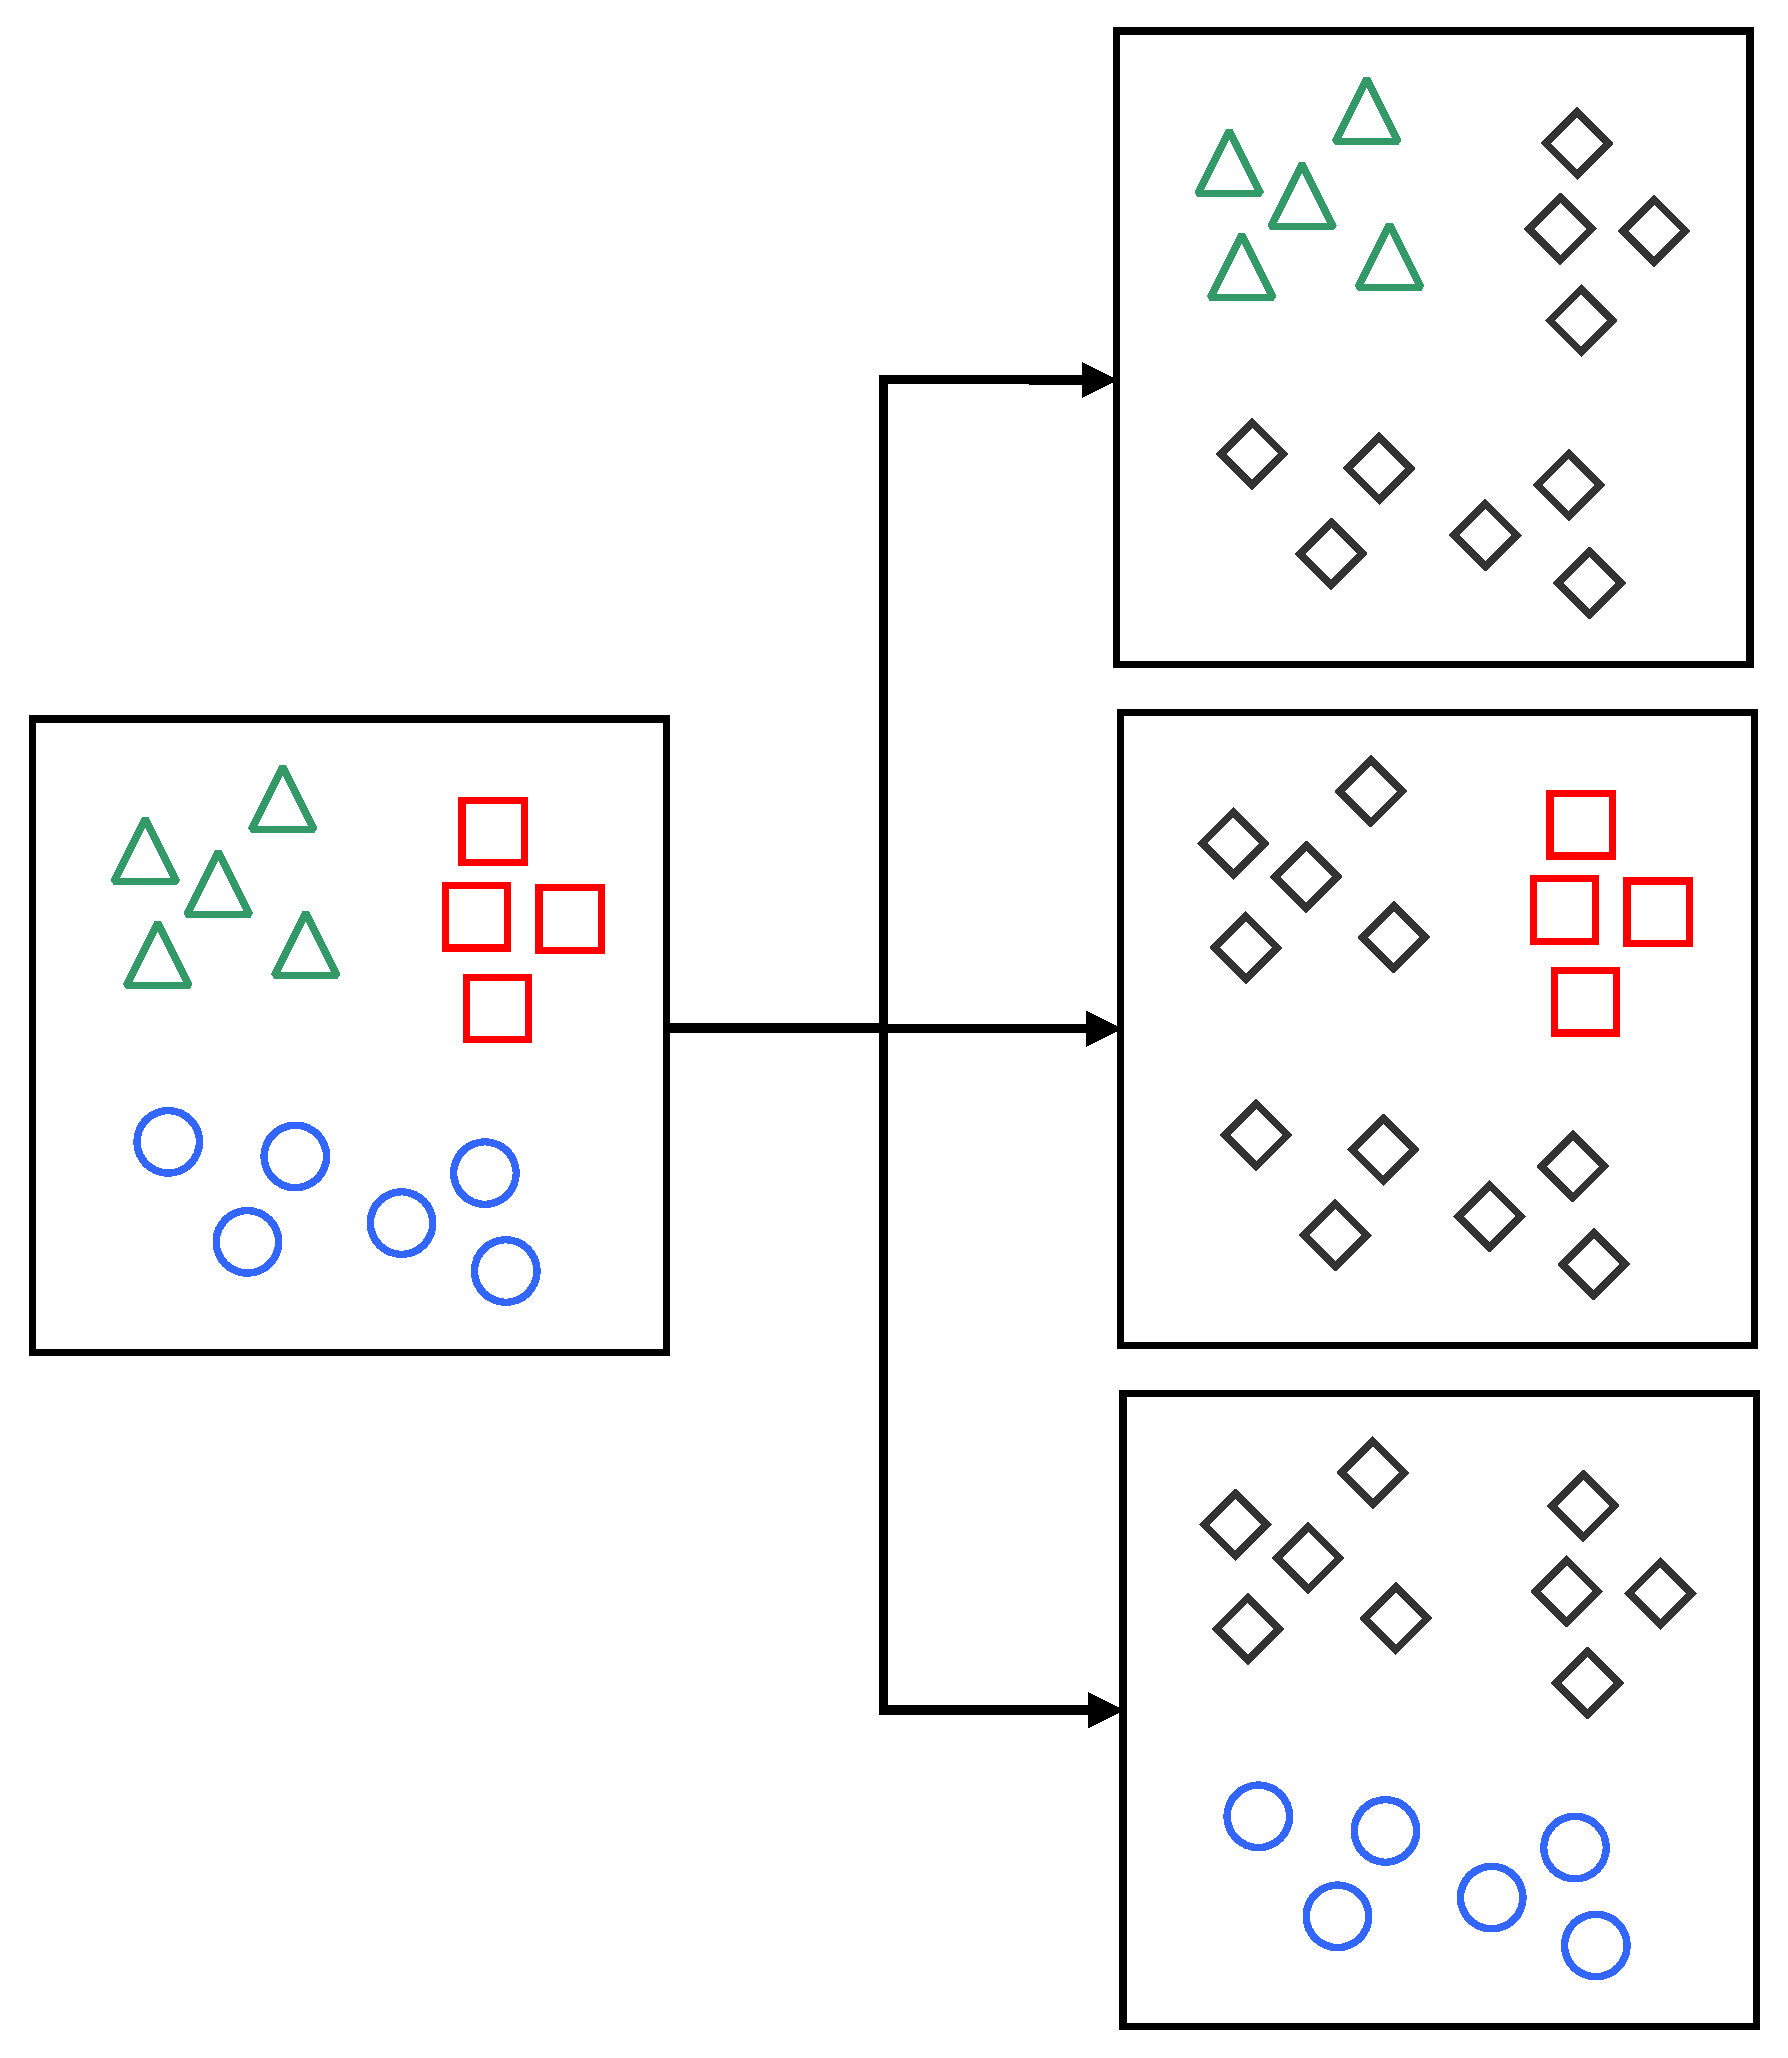
\includegraphics[width=0.5\textwidth]{Figures/one-vs-rest.pdf}
\decoRule
\caption[Algoritmo de One VS Rest]{Algoritmo de One VS Rest.}
\label{fig:ovr-algo}
\end{figure}

\todo[inline]{Pendiente: incluir arquitectura de solución en la \figureref{fig:model1-arch}}
\begin{figure}[H]
  \centering
  \missingfigure{Hacer la arquitectura en yEd}
  % 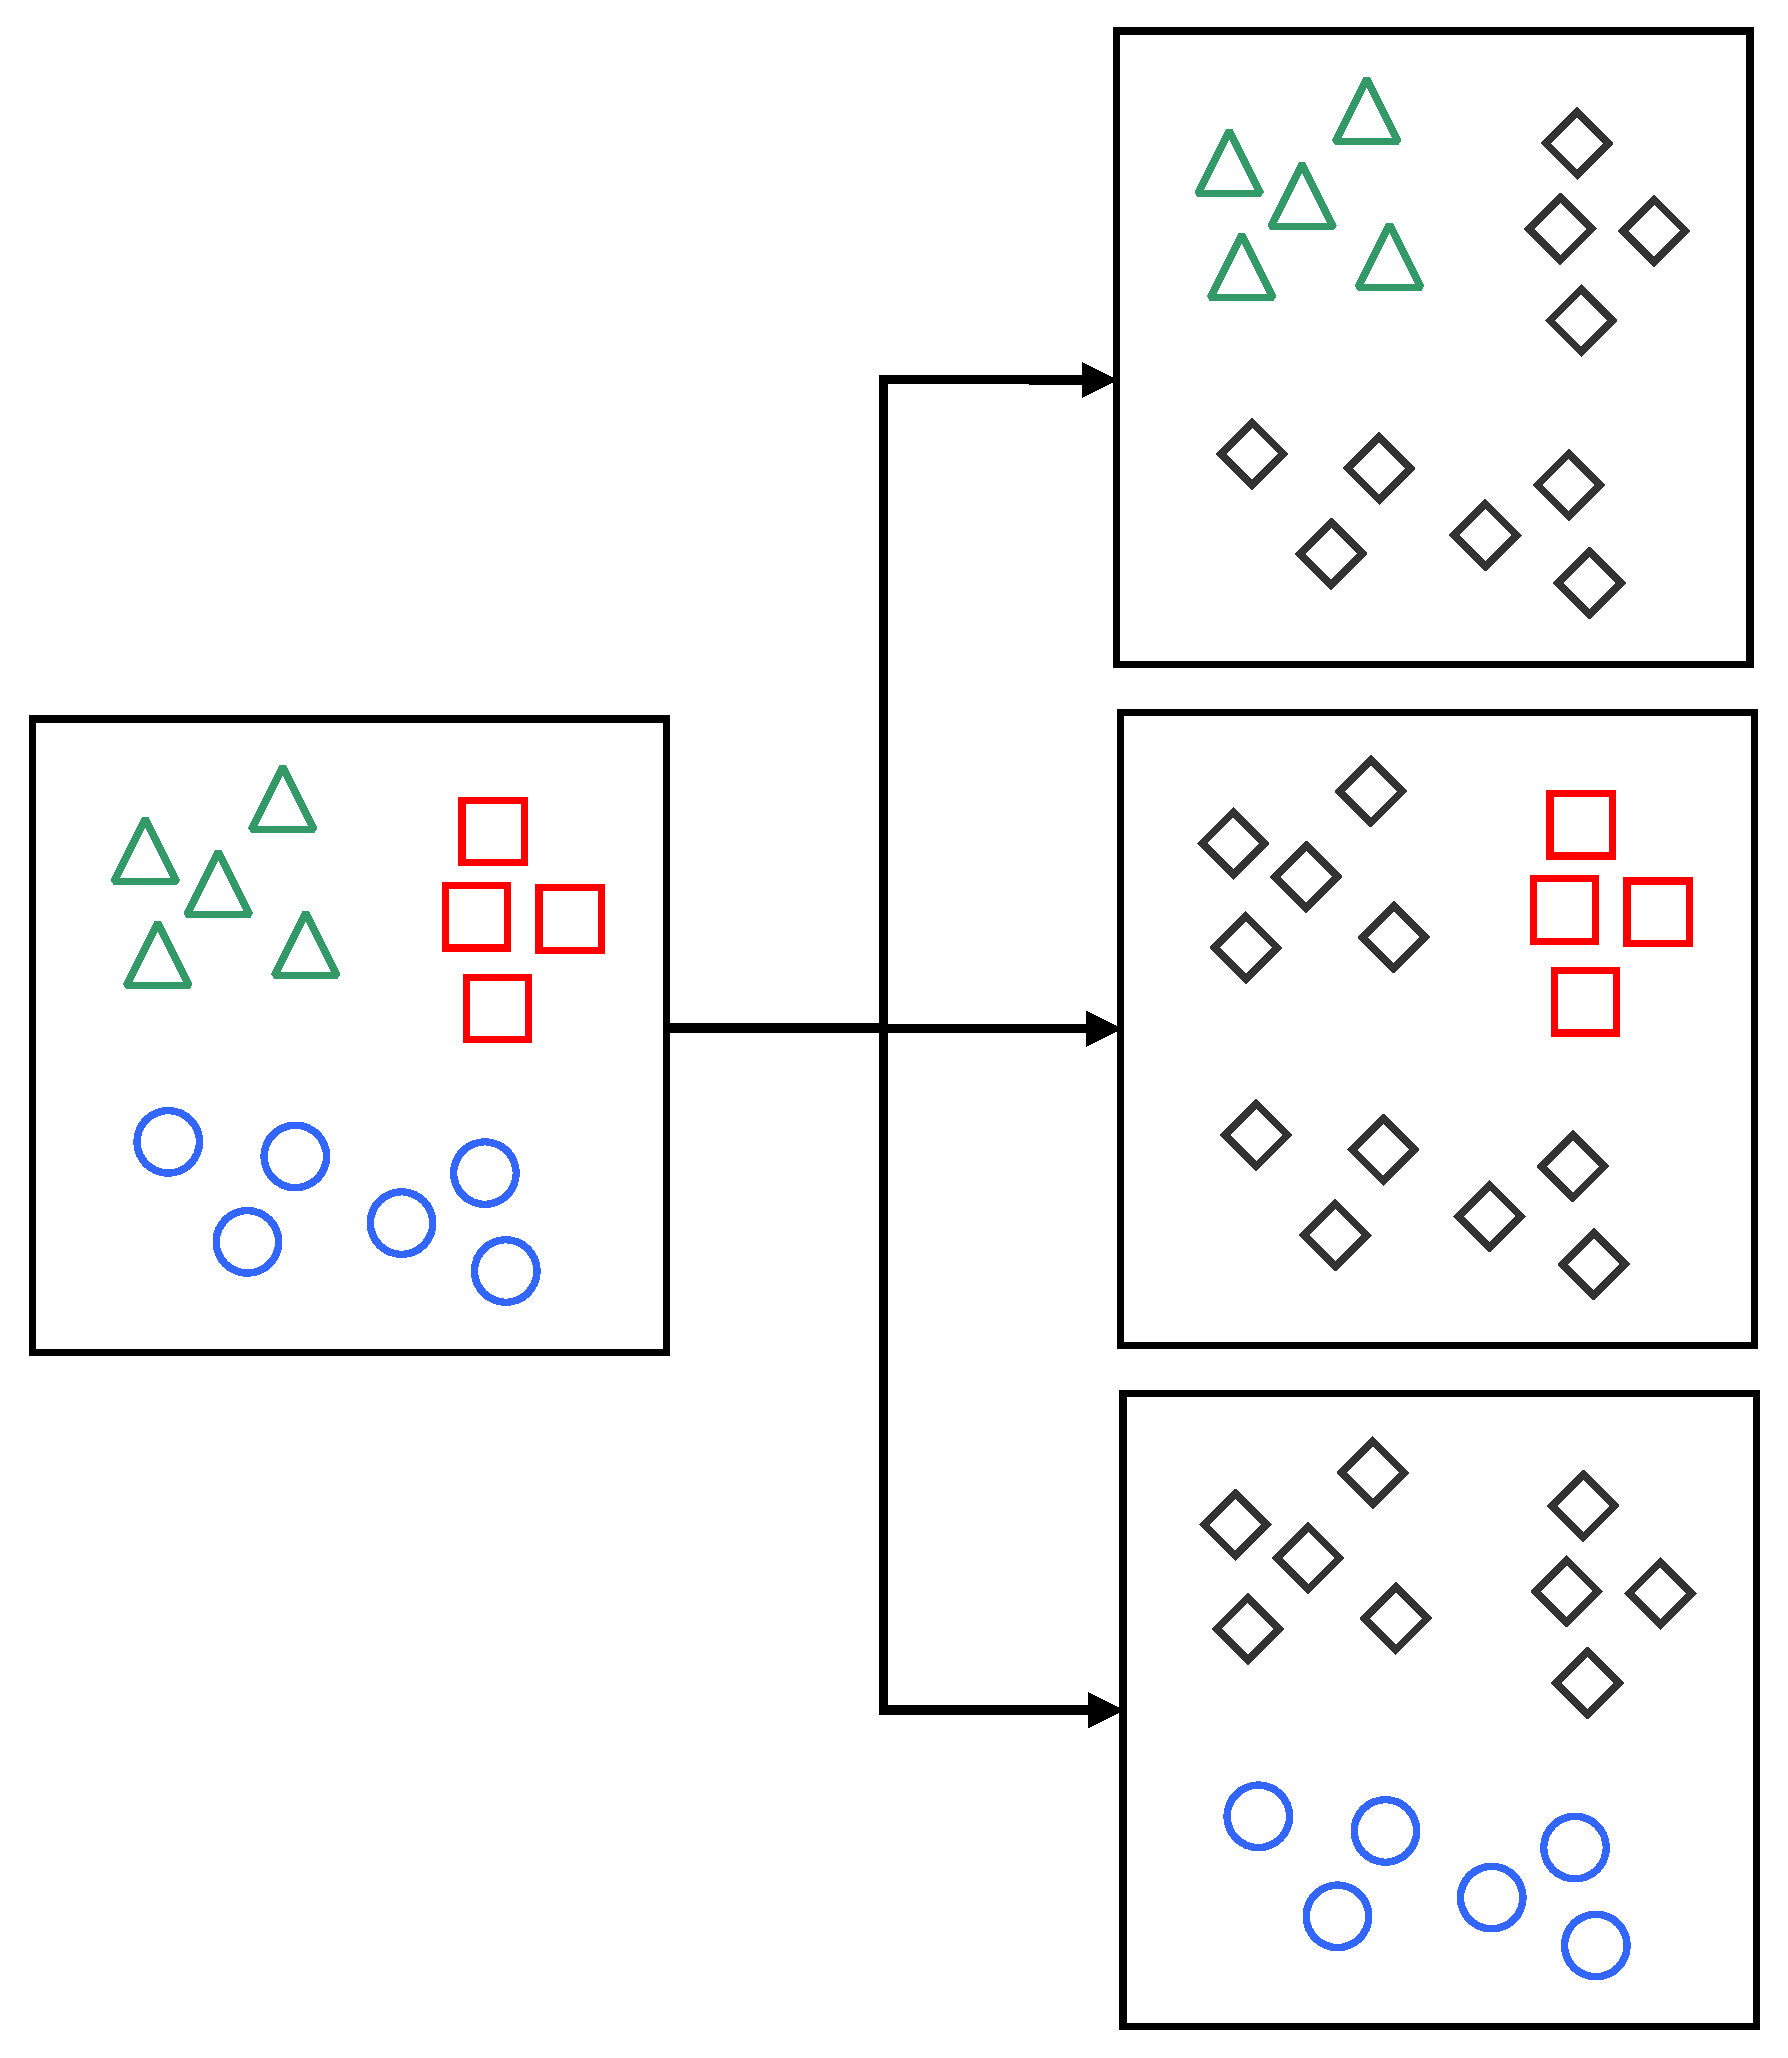
\includegraphics[width=0.5\textwidth]{Figures/one-vs-rest.pdf}
\decoRule
\caption[Arquitectura de Modelo 1]{Arquitectura de Modelo 1.}
\label{fig:model1-arch}
\end{figure}

%----------------------------------------------------------------------------------------

\subsection{Modelo 2: Reconocimiento de \glsentrylong{namedent} con redes \glsentrylong{lstm}}
\todo[inline]{Pendiente}
\todo[inline]{incluir diagramas de pagina de Google}

\subsection{Modelo 3: Búsqueda de tweets relacionados con \emph{embeddings} de \mbox{StarSpace}}
\todo[inline]{Pendiente}


\section{Despliegue (Deployment)}
\todo[inline]{Pendiente}
\lipsum{1}
